\begin{center}
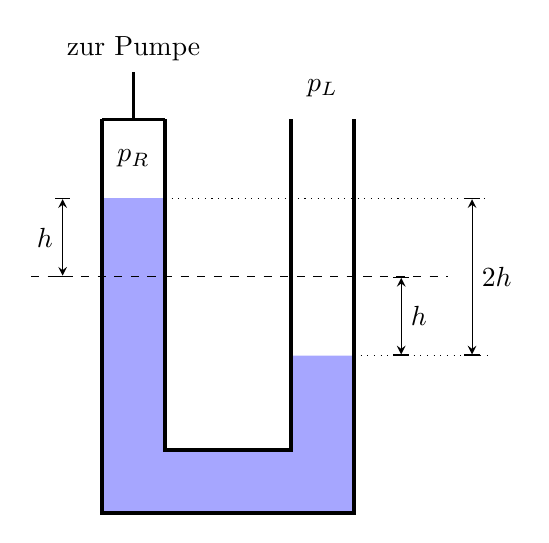
\begin{tikzpicture}[>=stealth]
 \fill[blue!35] (0,0) -- (0,4) -- (0.8,4) -- (0.8,0.8) -- (2.4,0.8) -- (2.4,2) -- (3.2,2) -- (3.2,0) -- cycle;
 \draw[very thick] (0,5) -- (0,0) -- (3.2,0) -- (3.2,5);
 \draw[very thick] (0.8,5) -- (0.8,0.8) -- (2.4,0.8) -- (2.4,5);
 \draw[very thick] (0,5) -- (0.8,5);
 \draw[very thick] (0.4,5) -- (0.4,5.6) node[above] {zur Pumpe};
 \node at (0.4,4.5) {$p_\text{R}$};
 \node at (2.8,5.4) {$p_\text{L}$};
 \draw[dashed] (-0.9,3) -- (4.4,3);
 \draw[dotted] (0.8,4) -- (4.9,4);
 \draw[dotted] (3.2,2) -- (4.9,2);
 \draw[|<->|] (-0.5,3) -- (-0.5,4) node[midway, left] {$h$};
 \draw[|<->|] (3.8,2) -- (3.8,3) node[midway, right] {$h$};
 \draw[|<->|] (4.7,2) -- (4.7,4) node[midway, right] {$2h$};
\end{tikzpicture}
\end{center}

Beide Schenkel haben denselben Querschnitt. Steigt der Spiegel auf der abgepumpten Seite um $h = \hstO$, so sinkt er auf der offenen Seite um gleich viel. Die Spiegel unterscheiden sich danach um
\begin{align}
 \Delta h &= \dhUF = \dhU
\end{align}
Auf der Höhe des tieferen Spiegels herrscht in beiden Schenkeln derselbe Druck:
\begin{align}
 p_\text{L} &= p_\text{R} + \rho\,g\cdot 2h
\end{align}
Mit dem Luftdruck $p_\text{L} = \pLO$ (Normaldruck) folgt
\begin{align}
 \rho &= \rhoUF \\
   &= \frac{\pL-\pR}{2\cdot\gE\cdot\hst} \\
   &= \rhoU \approx \result{\rhoUP{0}{2}}
\end{align}
Nach FoTaBe S.~187 ist das \result{\text{Quecksilber}} ($\rho_\text{Hg} = \rhoHgO$). Die kleine Abweichung kommt daher, dass der tatsächliche Luftdruck meist etwas kleiner ist als der Normaldruck.
